\section{Finally Big Data}

\subsection{Map Reduce Model}

\textbf{How can I scale the transformations to bilions of rows?}

MapReduce is a programming model proposed in a Google paper (2003)to easier multi-node process parallelization:

\begin{itemize}
	\item Users specify a map function that processes a key/value pair to generate a set of intermediate key/value pairs, and a reduce function that merges all intermediate values associated with the same intermediate key
	\item Programs written in this functional style are automatically parallelized and executed on a large cluster of commodity machines
	\item Inputs and operations over inputs are processed in parallel by different machines using a partitioning function (e.g., hash(key) mod R)
\end{itemize}  

\begin{center}
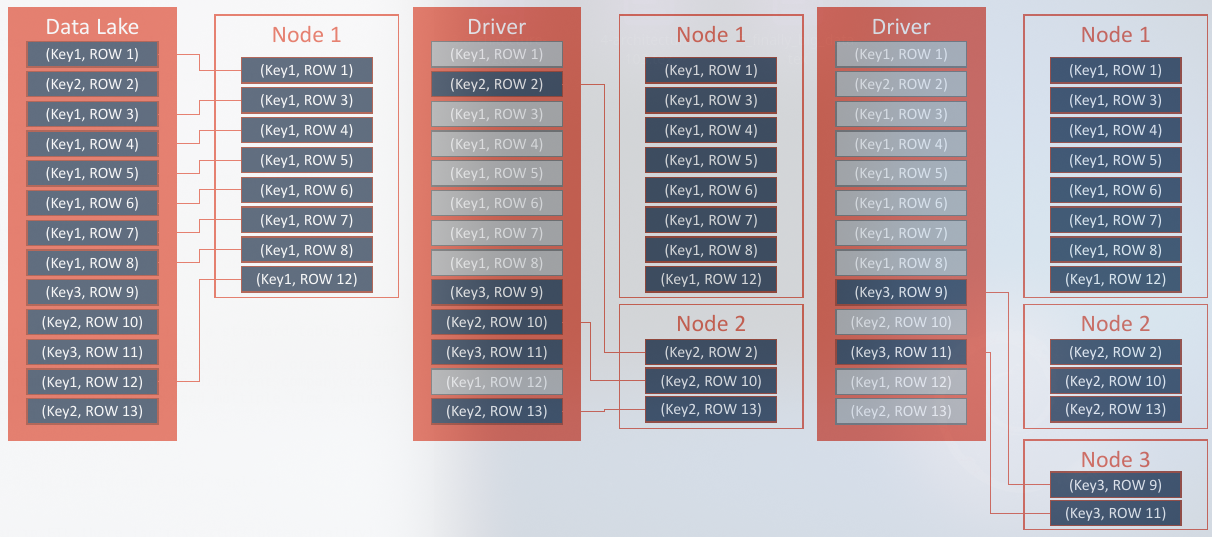
\includegraphics[scale=0.5]{51-map-reduce-model-1}
\end{center}

\begin{center}
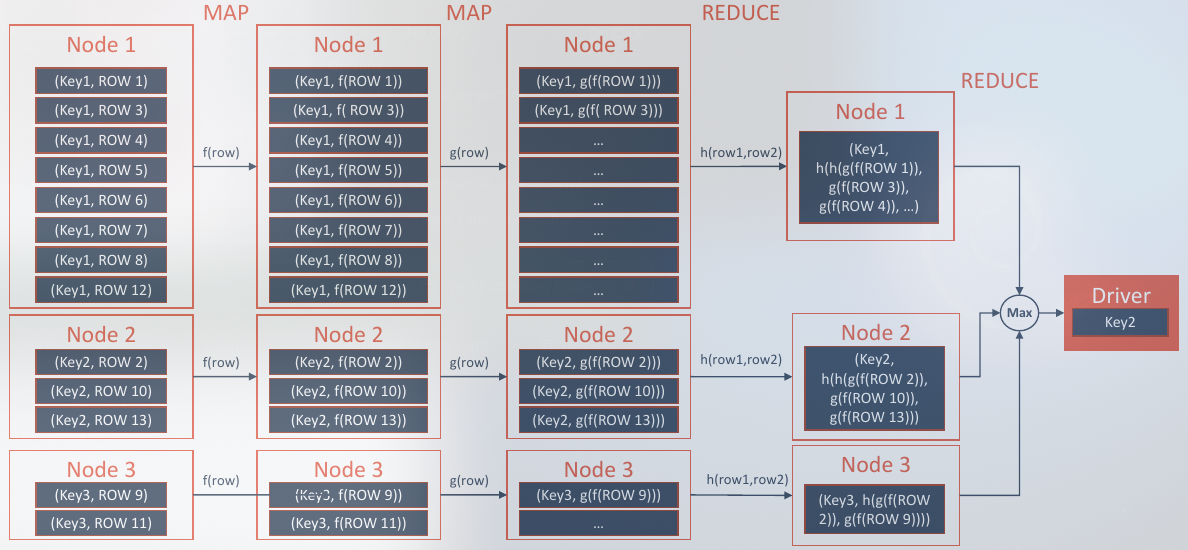
\includegraphics[scale=0.5]{51-map-reduce-model-2}
\end{center}

\subsection{Apache Hadoop}

\textbf{Distributed Parallel Frameworks}

\textbf{How to process data at scale}

\begin{itemize}
	\item Framework of -mostly- \textbf{open source components} built to facilitate the development of multi-node services written in Java
	\item Based on the assumption \textbf{hardware can fail}, several high reliability strategies are used inside Hadoop
	\item Three main components
	- \textbf{STORAGE} - Hadoop Distributed File System Storage (HDFS)
	- \textbf{RESOURCE MANAGEMENT} - Hadoop YARN
	- \textbf{PARALLEL COMPUTATION} - Hadoop MapReduce (implementation of Map Reduce pattern)
	\item Any Hadoop component should be location aware (name of the network switch where each node is) and should share it to the system to distribute data and computation
\end{itemize}

\subsubsection{Apache Architecture}

\begin{center}
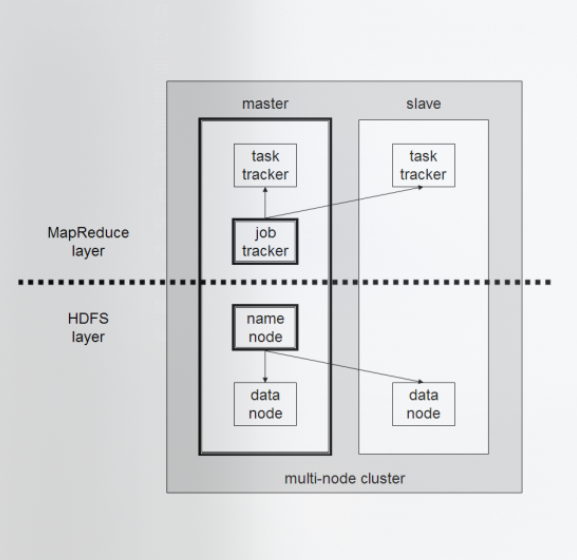
\includegraphics[scale=0.5]{52-hadoop-architecture-1}
\end{center}

\begin{itemize}
	\item \textbf{Job Tracker}
	- service that decide where a given task should be executed (ideally the nodes that have the data, or closer one)
	\item \textbf{Task Tracker}
	- a nde in the cluster that accepts tasks from a JobTracker. It expose a finite number of slots that represents its capability of run parallel tasks. Each task is executed on a spawned JVM. It also sends an heartbeat to the Job Tracker every minute to reassure it is still alive
\end{itemize}

\begin{itemize}
	\item \textbf{NameNode}
	- It keeps the directory tree of all files in the file system, and tracks where across the cluster the file data is kept. It does not store the data of these files itself. It is the Single Point of Failure of an Hadoop application. It routes request between application and DataNode
	\item \textbf{Backup NameNode}
	- Still under development to give to Hadoop High Availability
	\item \textbf{DataNode}
	- Stores data. DataNodes work with each other to replicate data. DataNode with data to process should be deployed on the same machine where TaskTracker is running
\end{itemize}

\begin{itemize}
	\item \textbf{Master Node}
	- Made by a Job Tracker, Task Traker, NameNode, and DataNode
	\item \textbf{Worker Node}
	- Made by a DataNode and TaskTracker
\end{itemize}


\subsubsection{Apache Sequence}

\begin{center}
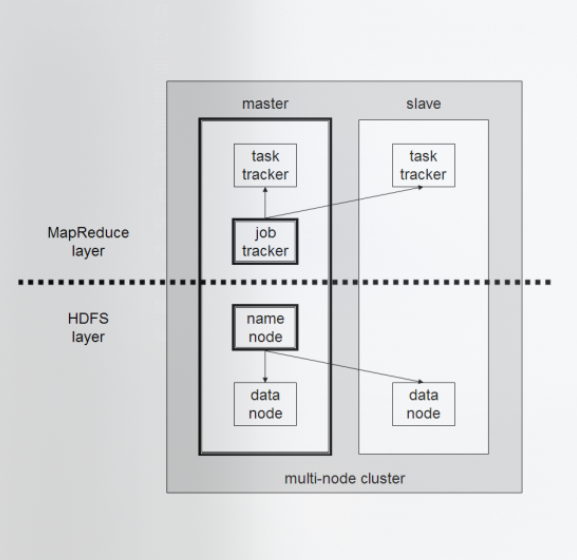
\includegraphics[scale=0.5]{52-hadoop-architecture-1}
\end{center}

\begin{itemize}
	\item Application submits an asyncronous job to the Job Tracker, then it can start polling the Job Tracker for job status
	\item Job Tracker gets data locations in the Name Node registry
	\item Job Tracker identifies the set of Task Trackers with available slots nearest to Data Nodes
	\item The JobTracker submits the work to the chosen Task Trackes
	\item ob Tracker starts to monitor Task Trackers heartbeat: If they do not submit heartbeat signals often enough, it presumes they failed and work is scheduled on a different Task Tracker.
	\item When each Task Tracker completes the task, it notify the Job Tracker the final status. If it failed, the Job Tracker can:
	1. resubmit the job elsewhere
	2. mark that specific record as to-skip
	3. blacklist the task traker as unreliable
\end{itemize}

\textbf{Moving computation is Cheaper than Moving Data}
A computation requested by an application is much more efficient if it is executed near the data it operates on. This is especially true when the size of the data set is huge. This minimizes network congestion and increases the overall throughput of the system. The assumption is that it is often better to migrate the computation closer to where the data is located rather than moving the data to where the application is running. HDFS provides interfaces for applications to move themselves closer to where the data is located.

\subsection{Hadoop Distributed File System Storage HDFS}

\textbf{HDFS is a distributed file syste designed to run on commodity hardware}

\begin{itemize}
	\item HDFS is highlt \textbf{foult-tolerant} and is designed to be deployed on low-cost hardware.
	\item HDFS provides \textbf{high throughput} access to application data and is suitable for applications that have large data sets.
\end{itemize}

\subsection{Hadoop YARN}

\textbf{YARN is based on the idea to split up the functionalities of resource management and job scheduling/monitoring into separate daemons}

\begin{itemize}
	\item Global ResourceManager (RM)
	ultimate authority that arbitrates resources among all the applications in the system
	\item [per-machine] NodeManager
	monitoring machine resource usage and reporting the same to the ResourceManager/Scheduler.
	\item [per-application] ApplicationMaster (AM)
	negotiating resources from the ResourceManager and working with the NodeManager(s) to execute and monitor the tasks.
\end{itemize}

\subsection{Hadoop Map Reduce}

\textbf{Hadoop MapReduce is a framework that implement MapReduce model taking care of scheduling tasks, monitoring them and re-executes the failed tasks.}

\begin{itemize}
	\item It consist of
	- a single master ResourceManager
	- one morker NodeManger per cluster-node
	- one AppMaster per application
	\item The Hadoop job client submits the job and configuration to the ResourceManager which then assumes the responsibility of distributing it to the workers
\end{itemize}

\subsubsection{Apache Sqoop}

Sqoop is a command-line interface application for transferring data between relational databases and Hadoop.

Sqoop supports incremental loads of a single table or a free form SQL query as well as saved jobs which can be run multiple times to import updates made to a database since the last import.

\textbf{Apache Sqoop (and CDC)}

\begin{center}
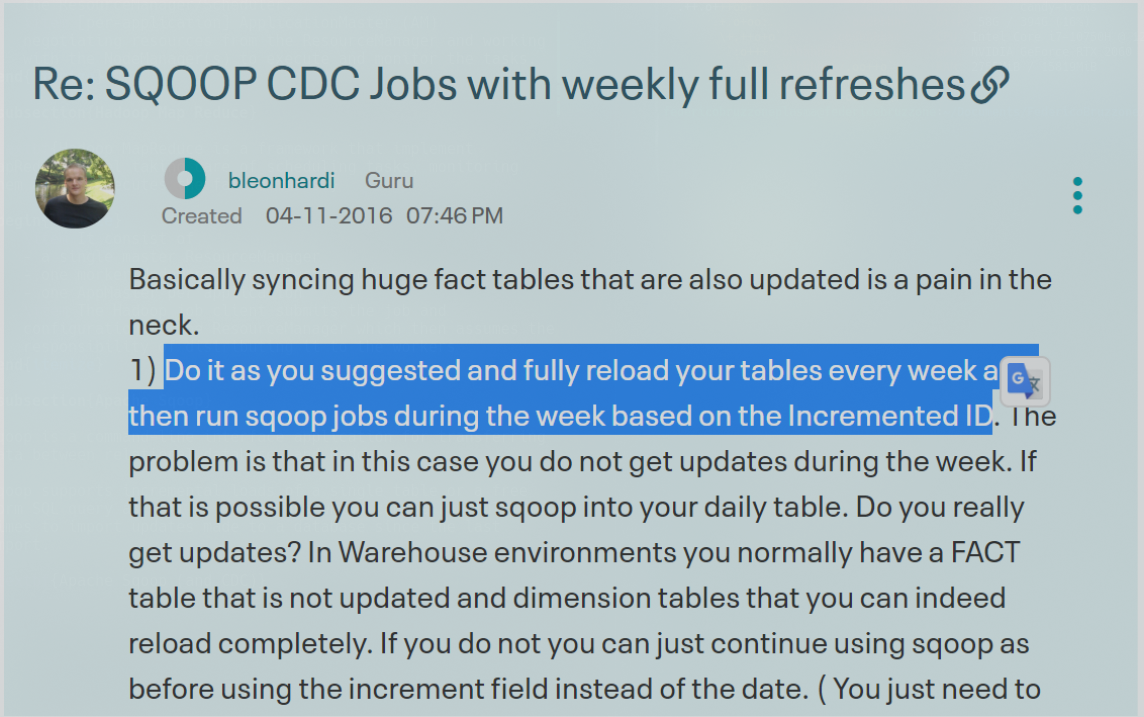
\includegraphics[scale=0.5]{53-apache-sqoop}
\end{center}

\subsubsection{Apache Hive}

Apache Hive is a data warehouse software project built on top of Apache Hadoop for providing data query and analysis.

Hive gives a SQL-like interface and a specific dialect HiveQL that is translated in Hadoop MapReduce jobs to query data.

Hive vs SQL:

Schema on Read         | Schema on Write

More efficient Write   | Less efficient Write

Less efficient queries | More efficient queries

\subsection{Data Lake over HDFS}

\subsubsection{Hadoop Architecture – HDFS}

\begin{center}
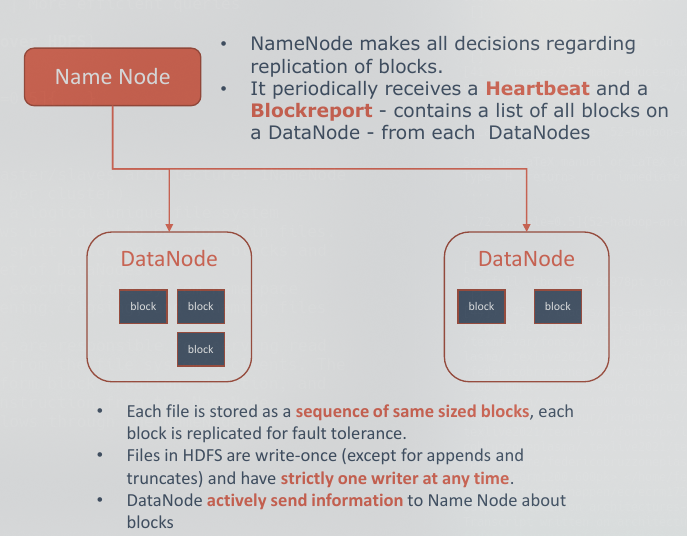
\includegraphics[scale=0.5]{54-hdfs-1}
\end{center}

\begin{itemize}
	\item HDFS has a master/slaves architecture: 1NameNode per n Datanodes (1 per cluster)
	\item HDFS exposes a logical unique file system namespace and allows user data to be stored in files.
	\item Each file is split into one or more blocks and distributed in a set of DataNodes.
	\item The NameNode executes file system namespace operations like opening, closing, and renaming files and directories.
	\item The DataNodes are responsible for serving read and write requests from the file system’s clients. The DataNodes also perform block creation, deletion, and replication upon instruction from the NameNode.
	\item Data never flows through the NameNode.
\end{itemize}

\textbf{HOW CAN WE WRITE WITH THOUSANDS OF SLAVES?}

\subsubsection{Hadoop Architecture – HDFS Replication Policy}

\begin{center}
\includegraphics[scale=0.5]{55-hdfs-2}
\end{center}

\begin{itemize}
	\item The NameNode determines the rack id each DataNode
	\item Placement of replicas are rack-aware to:

	- optimize network bandwidth

	- increase faoult tollerance

	- increase I/O performance
	\item Policy 1 – Replicate the entire rack Placement policy is to replicate the entire rack

	- prevents losing data if an entire rack fails

	- allows routing read requests over different racks optimizing network usage

	- Make easier re-load-balancing on component failure

	- increases the cost of writes because a write needs to transfer blocks to multiple racks.
\end{itemize}

\begin{center}
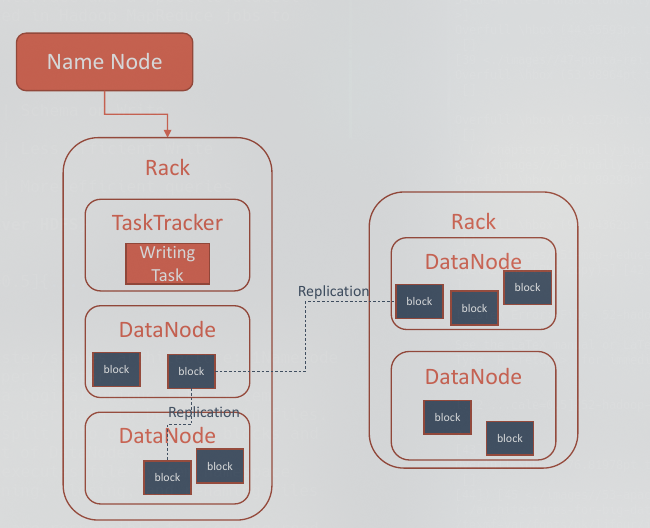
\includegraphics[scale=0.5]{56-hdfs-3}
\end{center}

\begin{itemize}
	\item Policy 2 – Two rack factor 3 replication Placement policy is to put one replica on a DataNode where the writer task is, another replica on a node in a different (remote) rack, and the last on a different node in the same remote rack.

	- Improved write performance: cuts the interrack write traffic

	- Sub-optimal reading: a block is placed in only two unique racks rather than three.

	- Sub-optimal file distribution:

		- one third of replicas are on one node,

		- two thirds of replicas are on one rack,

		- and the other third are evenly distributed across the remaining racks
\end{itemize}

\subsubsection{Hadoop Architecture - HDFS Replication Policy}

\textbf{DataNodes are reliable}
\begin{itemize}
	\item Each DataNode sends an Heartbeat message to the NameNode periodically.
	\item If a Datanode does not send an heartbeat before the long time-out – 10 minutes – ends it is considered death
	\item The NameNode constantly tracks which blocks need to be replicated and initiates replication whenever necessary.
\end{itemize}

\textbf{Data from DataNode is reliable}
\begin{itemize}
	\item It is possible that a block of data fetched from a DataNode arrives corrupted.
	\item The HDFS client software implements checksum checking on the contents of HDFS files computed on files creation and stored on HDFS itself
\end{itemize}

\textbf{NameNode could be reliable}
\begin{itemize}
	\item NameNode can be configured to support maintaining multiple copies of metadata and registry
	\item A distributed edit log could be used to add High Availability to NameNode - Quorum Journal Manager (QJM) feature.
\end{itemize}

\subsubsection{HDFS Quorum Journal Manager}

\begin{itemize}
	\item In a typical HA cluster, two or more separate machines are configured as NameNodes: exactly one is in an Active state, and the others are in a Standby state.
	\item A daemon write log any update on the active NameNode using daemons called “JournalNodes” (JNs)
	\item The active node is the only one able to write logs using Journal Nodes
	\item The Standby node is capable of reading the edits from the JNs, and is constantly watching them for changes to the edit log.
	\item DataNodes are configured with the location of all NameNodes (active and not), and send block location information and heartbeats to all.
	\item It avoid the so-called “split-brain scenario” the JournalNodes will only ever allow a single NameNode to be a writer at a time.
	\item During a failover, the NameNode which is going to become active will simply take over the role of writing to the JournalNodes
\end{itemize}

\subsubsection{Keep you data lake tidy!}


\begin{center}
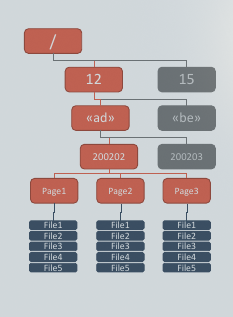
\includegraphics[scale=0.5]{57-keep-you-data-lanke-tidy}
\end{center}

\textbf{B-Tree+ could be used also when you design Data Lake objects structure}
\begin{itemize}
	\item Try to keep the same number of levels between root and data folders
	\item Enrich each line with the information about the path
	\item Keep the balance adding at the last level before leaves a new page if needed
	\item Each file should have same number of lines/object
	\item Each file should have a maximum size that depends on who is going to read them
	\item At each level, you could add a info.json file to describe some statistics about the rest of the path
	\item Even if you will always have a 1 page last layer, always add that layer: you will have a rule that does not depend on key values to end path recursion
\end{itemize}

\subsection{Arapche Spark - Deep Dive}

\subsubsection{Long Story Short}
\textbf{Netflix}
\begin{itemize}
	\item Apache Spark was created to support the Berkley team for the Netflix Prize
	\item It almost made it: same score but 20 minute of delay
	\item And this is why one of the first algorithm implemented was collaborative filtering (since 0.8.1)
\end{itemize}

\subsubsection{Apache Spark Architecture}

\textbf{How to connect Hadoop with Apache Spark}

\begin{center}
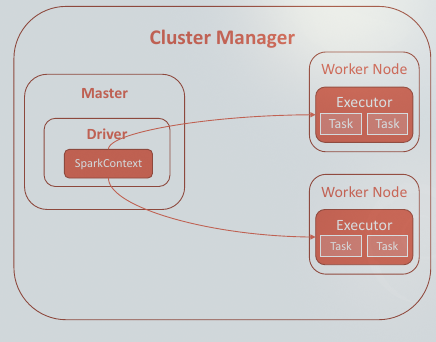
\includegraphics[scale=0.5]{58-apache-spark-architecture}
\end{center}
 
\textbf{Drive}
\begin{itemize}
	\item The driver is basically a process responsible for the execution of the spark application. 
	\item It is responsible for converting a user application into smaller execution units called tasks and then scheduling them.
	\item It holds the SparkContext, a singleton that allow to use Spark.
	\item Like NameNode, it stores metadata about all the Resilient Distributed Databases
\end{itemize}

\textbf{Master}
\begin{itemize}
	\item Is a framework-specific entity unique per application and responsible of negotiating resources with the ResourceManager and working with the NodeManager(s) to execute and monitor the component tasks.
	\item It will be sending resources request to the Resource Manager to get Worker Status.
	\item t is created on the same node of driver and could be back-upped in High Reliability configuration
\end{itemize}

\textbf{SparkContext}
\begin{itemize}
	\item Core Object for Apache Spark. It allows Spark Driver to use the cluster and call it through a Cluster Resource Manager.
	\item It’s the only way to create Spark specific type such as Resilient Distributed Dataset, Broadcast Variables, Accumulators.
	\item Spark Context also sends heartbeat message to executors to keeps track of executors status. It is created by Spark Driver inside Spark Driver JVM.
	\item It is a Singleton! (1 SparkContext per JVM) If you need to change JVM configuration, you must stop() and start() SparkContext.
\end{itemize}

\textbf{Worker}
\begin{itemize}
	\item Spark compute node where executors execute all the serialized tasks received in thread pools.
	\item It use a local Block Manager to communicate with other workers.
	\item When a SparkContext is created, each worker starts an executor as a separate process (JVM), and connects back to driver program to receive serialized code.
\end{itemize}

\textbf{Executors}
\begin{itemize}
	\item Distributed agent that is responsible for executing tasks.
	\item They enable the “Resilient” r of RDD: if one executor fail, all the task assigned are moved to another executor, and the task DAG is re-played on the new node.
	\item Task are tracked with a unique-id.
	\item Executors are also used to provide in-memory storage for RDDs when the user call the persist() or cache() method.
\end{itemize}

\subsubsection{Resilient Distributed Dataset}
\begin{itemize}
	\item The first Data Abstraction of Apache Spark is the Resilient Distributed Dataset (RDD)
	\item RDD is a collection of arbitrary elements partitioned across the nodes of the cluster with a hashPartitioner function
	\item RDDs are mainly created by starting reading objects from an HDFS file system (.textFile())
	\item RDDs could aslo been created “parallelizing” objects in memory (.parallelize())
	\item Default hashPartitioner function is applied to
	- a unique id built from files read
	- the row value casted to string after transformation if a re-shuffle is needed
	\item User can set the number of partitions (using .repartition(n)) to tune the parallelization
	\item An RDD made by a two elements tuple is called pairedRDD: in this case the hash function is applied to the first element of the tuple after any shuffle operation 
	\item If no custom hashPartitioner function is implemented, the default one is used: this  ensure same keys from different rdds are on the same node
\end{itemize}

\subsubsection{Paired– Resilient Distributed Dataset (PairedRdd)}

\begin{itemize}
	\item (key,value) version of RDD where
	- key can be everything could be serialized by your programming language
	- value can be everything could be serialized by your programming language
	\item The hashPartition function is applied to the value of "key"
	\item PairRDD are the only way to apply key-based transformations such as join or reduceByKey
	\item Playing with " key" you can enhance the performance of your system
	- Create a better distributed key
	- Force redistribution through repartition commands
\end{itemize}

\subsubsection{Shared Variables}

\begin{itemize}
	\item By default, when Spark distribute a function, it ships a copy of each variable used in the function once per row. This could lead to performance issue if the variables are big size maps or other complex structures.
	\item Spark supports two types of shared variables: broadcast variables, which can be used to distribute a read-only values once on all nodes, and accumulators, which which can be used to distribute a write-only variables.
	\item Accumulators are variables that are only “added” to through an associative and commutative operation and can therefore be efficiently supported in parallel. They can be used to implement counters (as in MapReduce) or sums.
	\item Broadcast variables allow the programmer to keep a read-only variable cached on each machine rather than shipping a copy of it with tasks. They can be used, for example, to give every node a copy of a large input dataset in an efficient manner. Spark also attempts to distribute broadcast variables using efficient broadcast algorithms to reduce communication cost.
	\item Spark actions are executed through a set of stages, separated by distributed “shuffle” operations. Spark automatically broadcasts the common data needed by tasks within each stage. The data broadcasted this way is cached in serialized form and deserialized before running each task. This means that explicitly creating broadcast variables is only useful when tasks across multiple stages need the same data or when caching the data in deserialized form is important.
\end{itemize}

\subsubsection{Spark is lazy!}

\begin{itemize}
	\item Spark is lazy: it does not compute their results right away. The computations happen only when the driver requires a result to be shown.
	\item Each transformation is recomputed each time a result is needed. However, trsanformation result may also be persisted in memory using .persist() method.
	\item Only the part of computation needed to show the required results are done (e.g., no tablescan if the first element is needed)
	\item Spark offers several Map functions. Each map function works line to rows-over-rows applying functions.
	\item Spark offers several Reduce functions. Such functions apply functions to couple of rows given a key untill there are no more couple of rows with the same key.
	\item Reduce functions must be commutative: no-one can know the exact order couple of rows are processed
	\item Good Spark Developers tries to avoid any kind of operations that requires rows distributed on different nodes: when this happens, it is called a Shuffle
\end{itemize}

\subsubsection{Transformations}

A transformations creates a new dataset from an existing one
No processing is done after a transformation is called.

\textbf{Available transformations:}
\begin{itemize}
	\item .map()
	\item .flatMap()
	\item .filter()
	\item .join(), .fullOuterJoin(), .rightOuterJoin(), leftOuterJoin()
	\item .reduceByKey()
	\item .repartition()
	\item .cartesian()
\end{itemize}

\subsubsection{Actions}
Actions return a value to the driver program after running a computation on the dataset.

\textbf{Available actions:}
\begin{itemize}
	\item .first()
	\item .take(n)
	\item .top(n,key)
	\item .collect()
	\item .count()
	\item .stats()
\end{itemize}

\subsubsection{From RDD to workers}

\begin{center}
  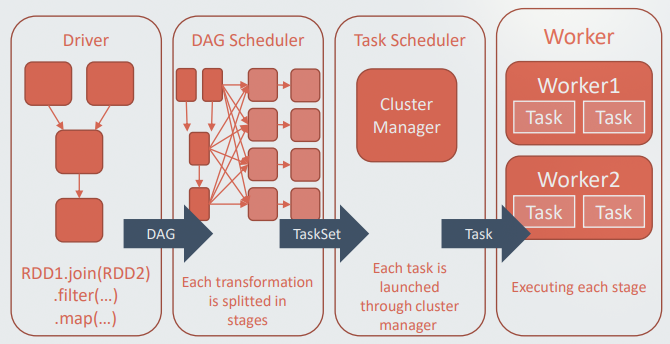
\includegraphics[scale=0.5]{59-from-rdd-to-workers}
\end{center}

\begin{itemize}
  \item Any trasformation made over an RDD just adds nodes to a Direct Acyclic Graph (DAG)
  \item DAGScheduler recives the a logical execution plan (the DAG) and transform it into a physical execution plan
  \item Execution plan is composed by a DAG of stages that implement the transormation logic
  \item A Stage executed over a specific group of rows is called task
  \item The TaskScheduler launches tasks via the cluster
  \item The number of tasks submitted sepends on the number of partitions in which actually is splitted the RDD
  \item Workers execute task
\begin{itemize}

\subsubsection{Visual textFile, (map), repartition, persist, and count}
\begin{center}
  \includegraphics[scale=0.5]{60-repartition}
\end{center}

\subsubsection{Common pipeline - T:textFile, T:map, T:filter: A:count}
...
\subsubsection{Count a distribution}
...
\subsubsection{Transformation- rdd.reduceByKey(lambda val1, val2: f(val1, val2))}
...
\subsubsection{Commutative reduction}
...
\subsubsection{rdd.filer()}
...
\subsubsection{Get closest element}
...

